% !TeX spellcheck = ru_RU
\section*{Приложение А}

\begin{table}[h]
\centering
\small
\caption{Сравнение библиотек для парсинга и NER}
\begin{tabularx}{\textwidth}{|X|X|X|X|}
\hline
\textbf{Библиотека} & \textbf{Назначение} & \textbf{Плюсы} & \textbf{Минусы} \\
\hline
Requests + BeautifulSoup & парсинг HTML & лёгкость, широкое сообщество & требуется ручной разбор тегов \\
\hline
spaCy (ru\_core\_news\_sm) & NER & быстрая, предобучена на русском & может ошибаться на фандомных именах (классифицирует как LOC) \\
\hline
Natasha & NER & альтернатива, хороша для русского & требует отдельной установки, не превзошла spaCy \\
\hline
PostgreSQL & хранение данных & внешние ключи, стандартный SQL & нужна настройка импорта CSV \\
\hline
NetworkX + matplotlib & визуализация графов & мощные, гибкие & статичные (не интерактивны) \\
\hline
\end{tabularx}
\normalsize
\label{tab:comparison}
\end{table}


\section*{Приложение Б}

\begin{figure}[h]
\centering
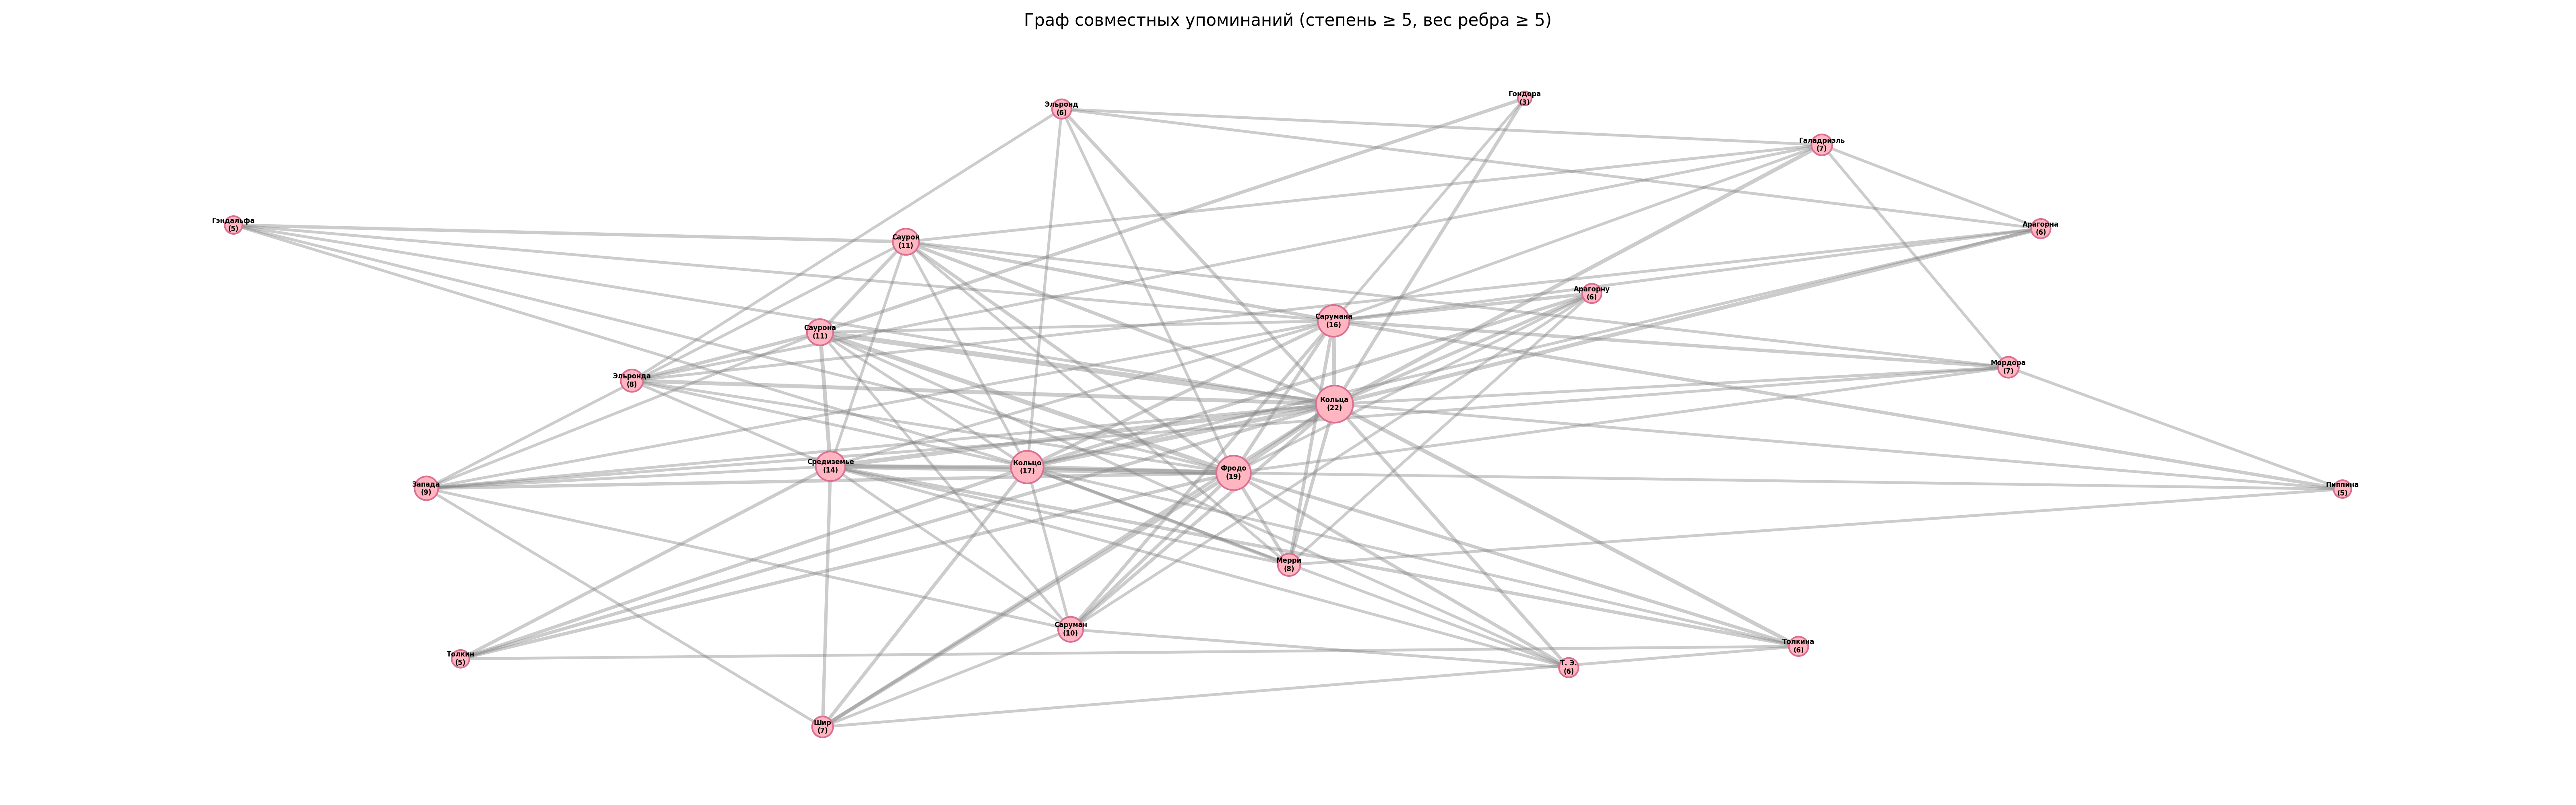
\includegraphics[width=1.0\textwidth]{figures/graph.png}
\caption{Граф совместных упоминаний персонажей (степень >= 5, вес ребра >= 5)}
\label{fig:graph}
\end{figure}